%
%  Wakefield Acceleration
% ========================
%

\chapter{A Wakefield Accelerator Experiment}
\label{Ch:WFA}

AWAKE is the first proton driven wakefield accelerator experiment in the world. It is a proof-of-concept experiment aiming to inform a design for future high energy accelerators \cite{gschwendtner:2016}. The proton drive beam is delivered by the Super Proton Synchrotron (SPS) at CERN. The experiment is physically located at the former site of the CERN Neutrinos to Gran Sasso experiment (CNGS) \cite{gschwendtner:2010} in a tunnel below the Swiss-French border connected to the SPS at SPS Point 4. The placement of the AWAKE experiment in relation to the rest of the CERN accelerator complex can be seen in Figure \ref{Fig:WFA:AccComp}.

\begin{figure}[hbt]
    \centering
    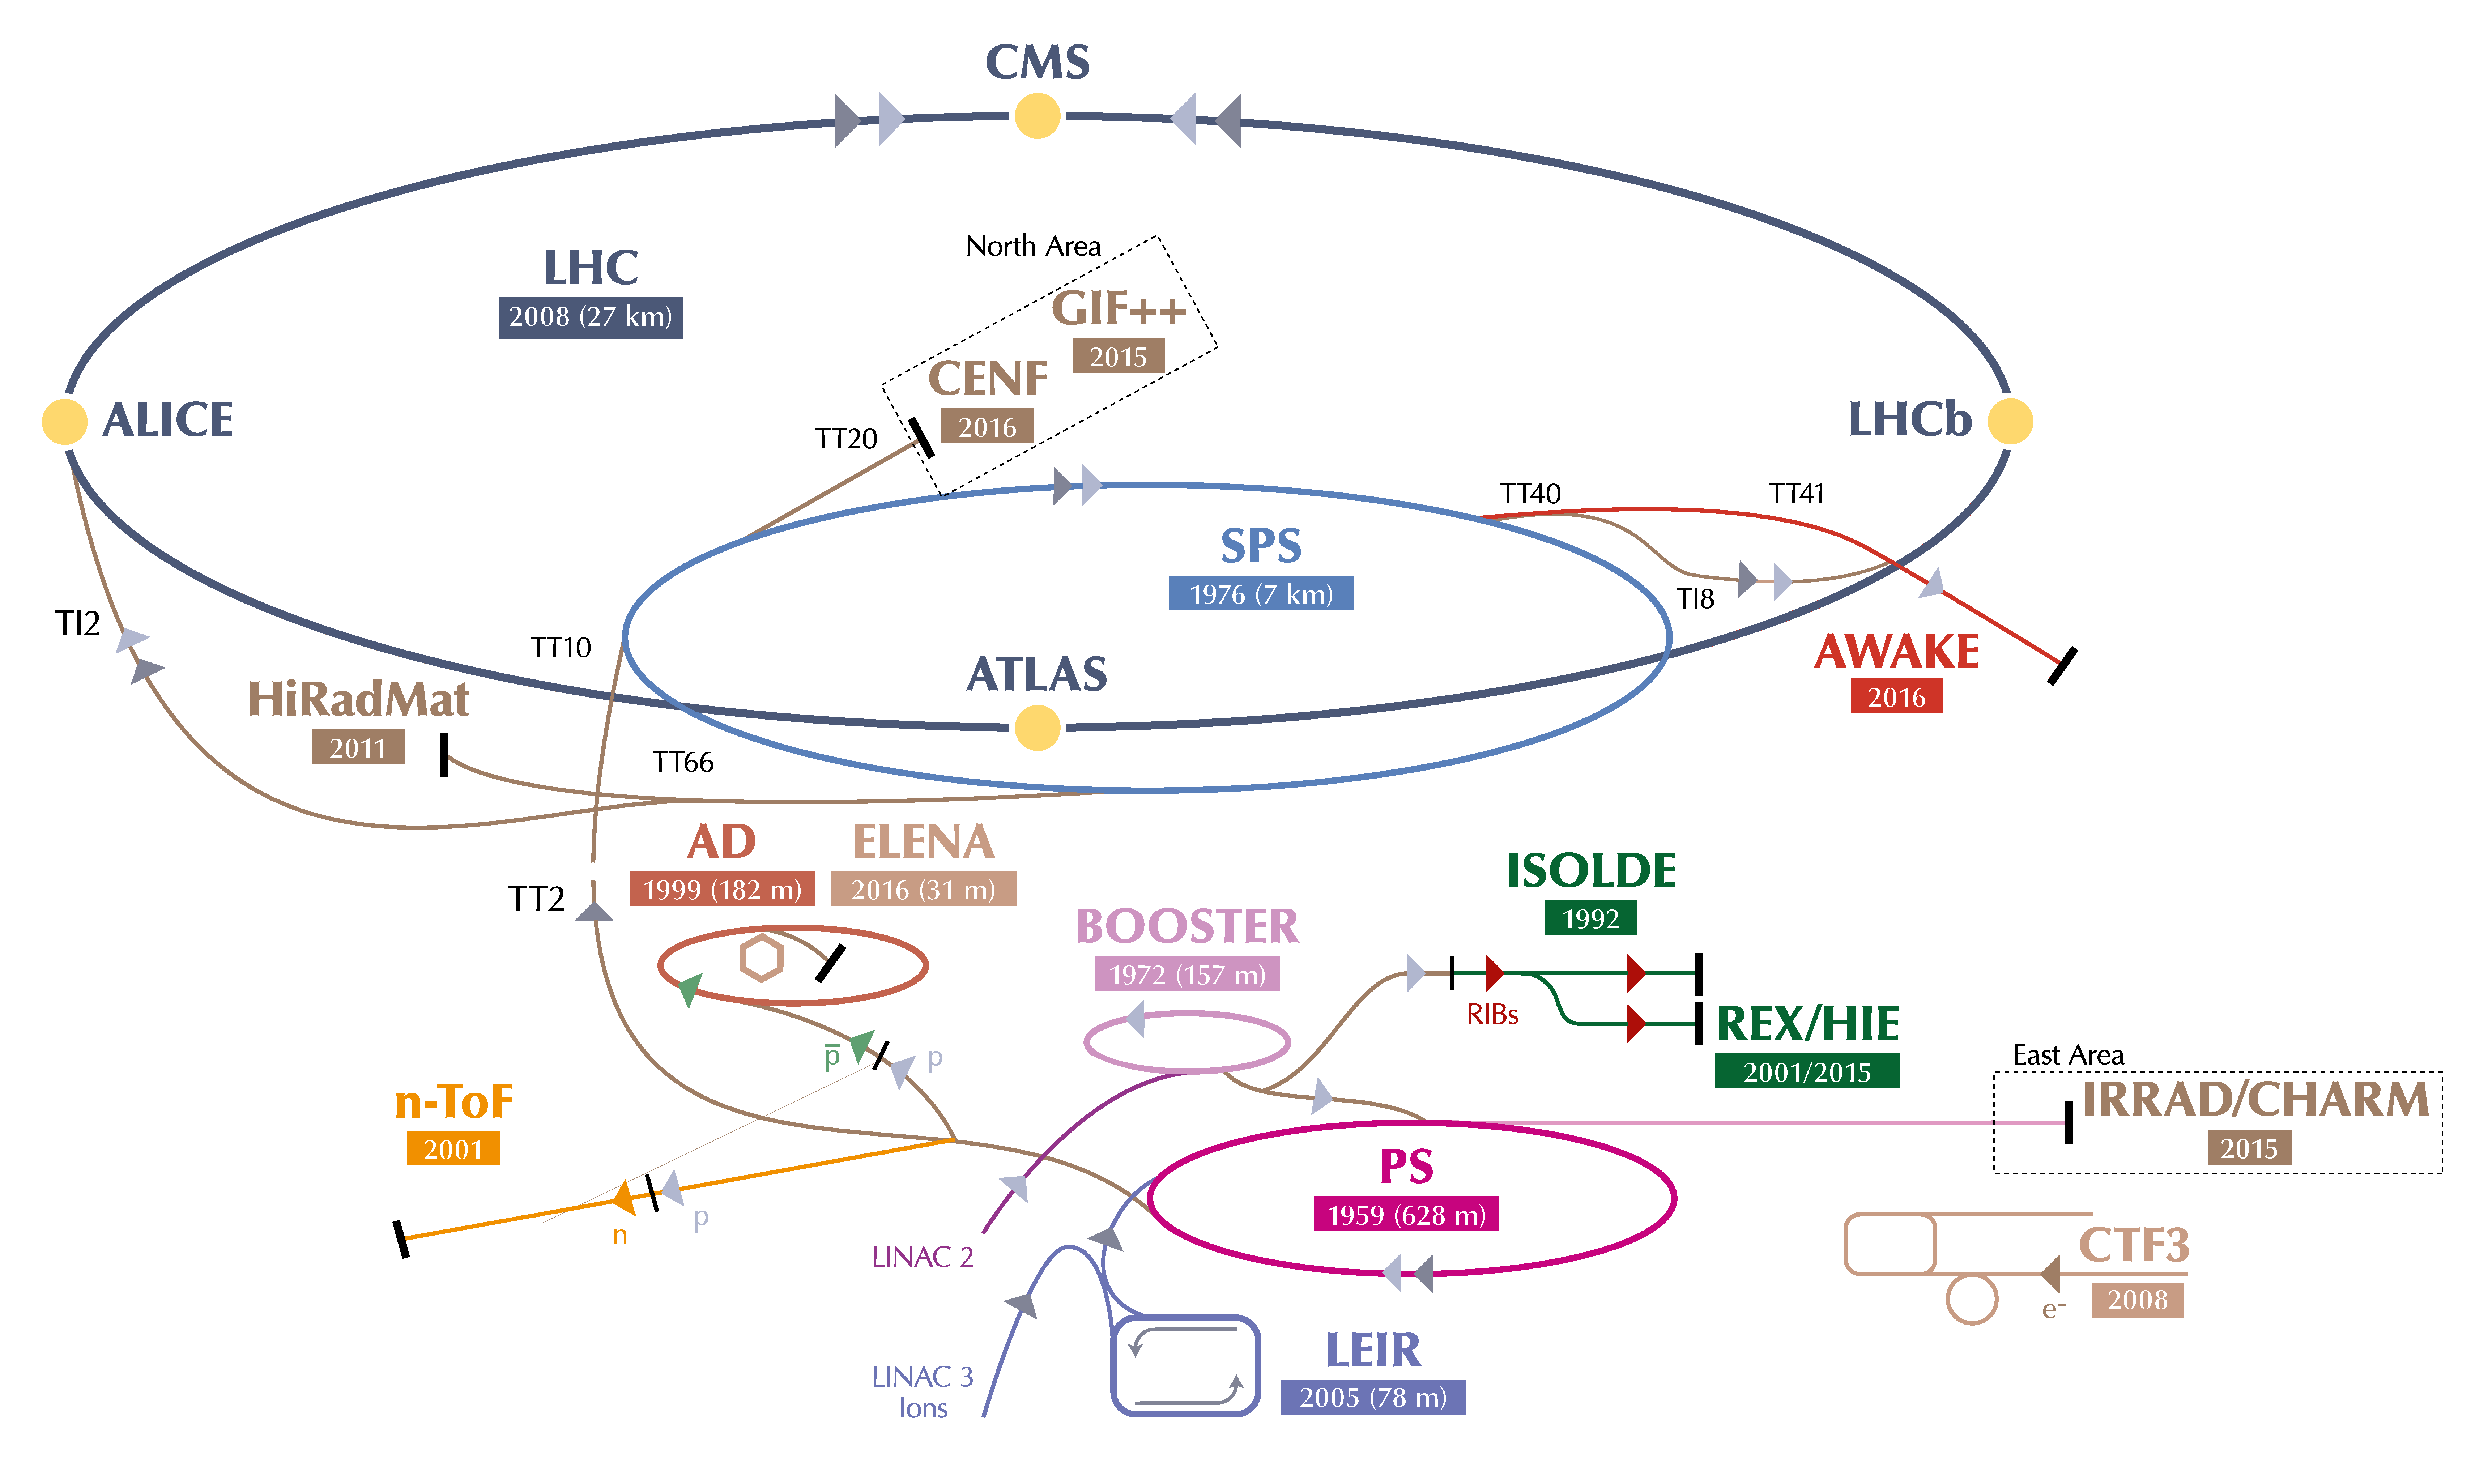
\includegraphics[width=0.99\linewidth,trim={20mm 0mm 20mm 0mm},clip]{figures/AcceleratorComplex}
    \caption{\label{Fig:WFA:AccComp} An overview of the CERN Accelerator Complex \cite{add:mobs:2016}.}
\end{figure}



Intro paper \cite{caldwell:2009}

Launch paper \cite{awake_collaboration:2014}

Evolution paper \cite{caldwell:2016}

Technical specs including simulation parameters \cite{gschwendtner:2016}

Status report \cite{awake_collaboration:2016}

% ================================================================================================ %
\section{Evolution of the Concept}
\label{WFA:History}

Previous experiments, SLAC, etc.

\cite{rosenzweig:1988, blumenfeld:2007, kallos:2008, litos:2014}

Self modulation at FACET \cite{adli:2016}

Review by Patric \cite{muggli:2009}

% ================================================================================================ %
\section{The Advanced Wakefield Experiment (AWAKE)}
\label{WFA:AWAKE}

A summary of the AWAKE experiment

% ================================================================================================ %
\subsection{AWAKE Run 1}
\label{WFA:AWAKE:R1}

\begin{table}[hbt]
    \centering
    \caption{Nominal AWAKE experiment beam parameters for Run 1 \cite{gschwendtner:2014, gschwendtner:2016}.}
    \label{T:AWAKE-Run1}
    \begin{tabular}{lll}
        \hline
        \textbf{Parameter} & \textbf{Proton Beam} & \textbf{Electron Beam} \\
        \hline
        Momentum &
            $400\unit{GeV}$               & $16\unit{MeV}$ \\
        Charge &
            $4.8\unit{nC}$                & $200\unit{pC}$ \\
        Particles &
            $3\nexp{11}$                  & $1.25\nexp{9}$ \\
        Bunch length ($\sigma_{z}$) &
            $12\unit{cm}\;(0.4\unit{ns})$ & $1.2\unit{mm}\;(4\unit{ps})$ \\
        Bunch size ($\sigma_{x,y}$) &
            $200\unit{\mu m}$             & $250\unit{\mu m}$ \\
        Normalised emittance ($\emitN$) &
            $3.5\unit{\mu m}$             & $2\unit{\mu m}$ \\
        Relative energy spread ($\Delta p/p$) &
            $0.035\%$                     & $0.5\%$ \\
        Beta function ($\beta^{*}_{x,y}$) &
            $4.9\unit{m}$                 & $0.4\unit{m}$ \\
        Dispersion ($D^{*}_{x,y}$) &
            $0$                           & $0$ \\
        \hline
    \end{tabular}
\end{table}

Description of Run 1. SMI, long e-beam.

% ================================================================================================ %
\subsection{AWAKE Run 2}
\label{WFA:AWAKE:R2}

Short e-beam, multiple stages, etc.

Problems relevant for this thesis.

Erik \cite{adli:2016a}

% ================================================================================================ %
\section{The Self-modulation Instability in AWAKE}
\label{WFA:SMI}

Results from Run 1 of the experiment.

% ================================================================================================ %
